

\section{深夜徘徊のすすめ}
文責:雁音
\subsection{はじめに}
入寮パンフを手に取ってくださったみなさま、特にこの記事に目をとめてくれたみなさま、お読みいただきありがとうございます。今年はどんな記事が寄稿されているのでしょうか。入寮パンフに文章を載せていただくのは今回が初めてなので、すこし肩肘を張っているかもしれませんが、どうか最後までお目通しいただければ幸いです。\\ \indent 
さて、熊野寮には数多くの趣味コミュニティが存在しますが、そのひとつに深夜徘徊部があります。深夜徘徊というと、夢遊病かのような印象のある語彙ですが、実態としては「深夜散歩」なんかが近いです。目的地がなかったり、ありえない距離を歩いていたり、結果帰寮が朝だったりするので、かえって散歩より徘徊の方がニュアンスが適切かもしれません。とかく、僕たちの趣味たる深夜徘徊について魅力を伝えられたらなと思い、発案に至りました。\\ \indent 
京都という街は深夜徘徊に本当に適しています。京都に惹かれて京大を受けた、そこの非関西勢!僕と同じですね。ぜったいにハマるので、入寮した暁には、ぜひとも一緒に行きましょう。

\subsection{本編}
あらためて、はじめまして。入寮3年目の雁音といいます。3年目って本当ですか…?全然実感がない、まだ2年目くらいの気分。かるく自己紹介をすると、緑茶とスマブラとピアノと哲学と化学が好きな人です。それぞれ話すと大変なことになってしまうので、入寮面接や入寮後にお話しする機会があればということで。深夜徘徊には入学して一か月後くらいには行き出していたのですが、ひとと行くようになったのは実は最近なんですよね。雑談の機会としては勿論、自分と違う視点で街の解釈を語ってくれるのもとっても愉快です。熊野寮は全体的に話し合いが実に盛んな場所です。それは運営方針の擦り合わせやトラブルの解決という分かりやすい手段に留まることなく、談話室の存在による日常的な対話の多さや、一緒に生活を営み、お互いの解像度が上がることによる立ち入る内容の深さが特徴的な文化となっています。それがゆえに、寮生は話の構成や言語化が上手だったり、自分の好きな分野への熱意や知識量が豊富だったりして(これは京大全体に言えるかもしれませんね)、とかく話していて楽しいです。\\ \indent
少し話が逸れました。以下では、深夜徘徊の何が好きなのか言語化すること、好きな写真から語ることに分けて発信していこうと思います。どのくらい長くなるか分かりませんが、しばしお付き合いいただければと思います。\\ \indent
\subsection{何が好き?}
深夜徘徊の魅力を「深夜」と「徘徊」の要素に分解してみます。まずは「深夜」から。分かりやすい点から行くと、人が少ない!これは本当に魅力的です。過剰なひとごみが苦手で、さらに言えば、それがゆえに景色の本来の姿が見えなくなることが悲しい僕としては、深夜の人の少なさにはかなり救われるものがあります。夜の景色は(昼の景色に対し、多くの場合で)本来的ではないと言われてしまうとその通りなのですが、体感としては、昼夜というワンセットは「自然の」摂理としてそこにあるので、夜の景色も見つめたいなあと思っています。これに関連して、根本的に深夜はものが見えにくいので、意識しないものを見ずにいられるというのも良いですね。深夜だとニュートラルに流れ込む情報量が少ないので、考え事をしたり、ひとと腰を据えて(歩いていますが、)話したりする上で良く作用します。もちろん、単に落ち着くというのもありますね。\\ \indent
「徘徊」については、散歩と魅力の多くが共通していると思います。より正確に言うと、目的のない散歩です。たくさん歩くのって楽しいですよね。運動不足がちな寮生においては健康にも寄与しています(昼であればより健康…)。熊野寮には「エクストリーム帰寮」という寮祭企画があります。目隠しをして車に乗り、寮から遠く(20km~100kmが標準的?)に飛ばされ、徒歩で帰寮するというコンセプトの企画です。これと同じように、意味不明な目的地を設定したりしなかったりして、長距離を歩くというのは僕を惹いて止みません。地球上どこでもそうですが、特に京都で顕著なこととして、長距離を歩くと街並みの変遷が実感できて面白いということがあります。京都の街並みが好きで進学した場合はなおのこと!ひとと歩く場合ならば、街を題材に話のネタが尽きないというのも地味に推しポイントです。\\ \indent

\subsection{好きな写真たち}
\begin{figure}[H]
    \centering
    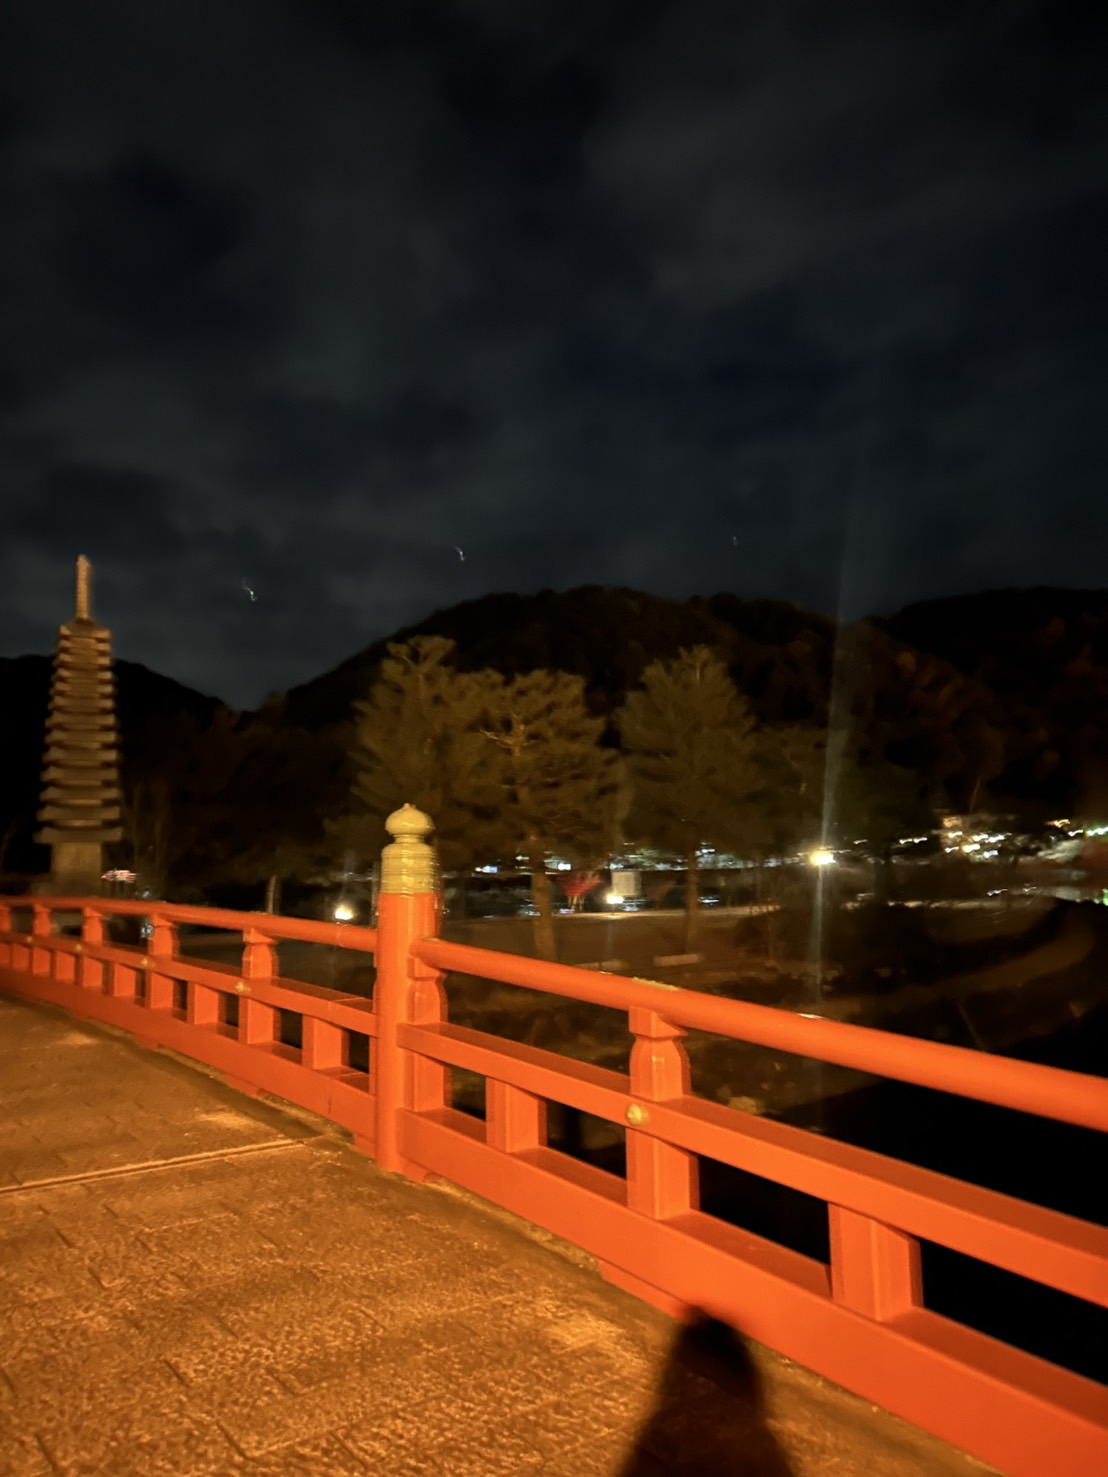
\includegraphics[width=5cm]{2025shinki/shinya_haikai/image1.png}
    \caption{@宇治公園}
    \label{fig:enter-label1}
\end{figure}

深夜と朱色ってめちゃくちゃ良いんですよね。京都には朱色が多くて、うれしい限りです。静寂の宇治公園の中では川の流水音も聞こえるのですが、これもたまらない。安易に歩いて行くには
遠すぎるという点を除けばきわめて好みのスポットです。印刷だと白黒になってる気がする、というか悪くすると真っ黒になっている…?祈るばかりです。

\begin{figure}[H]
    \centering
    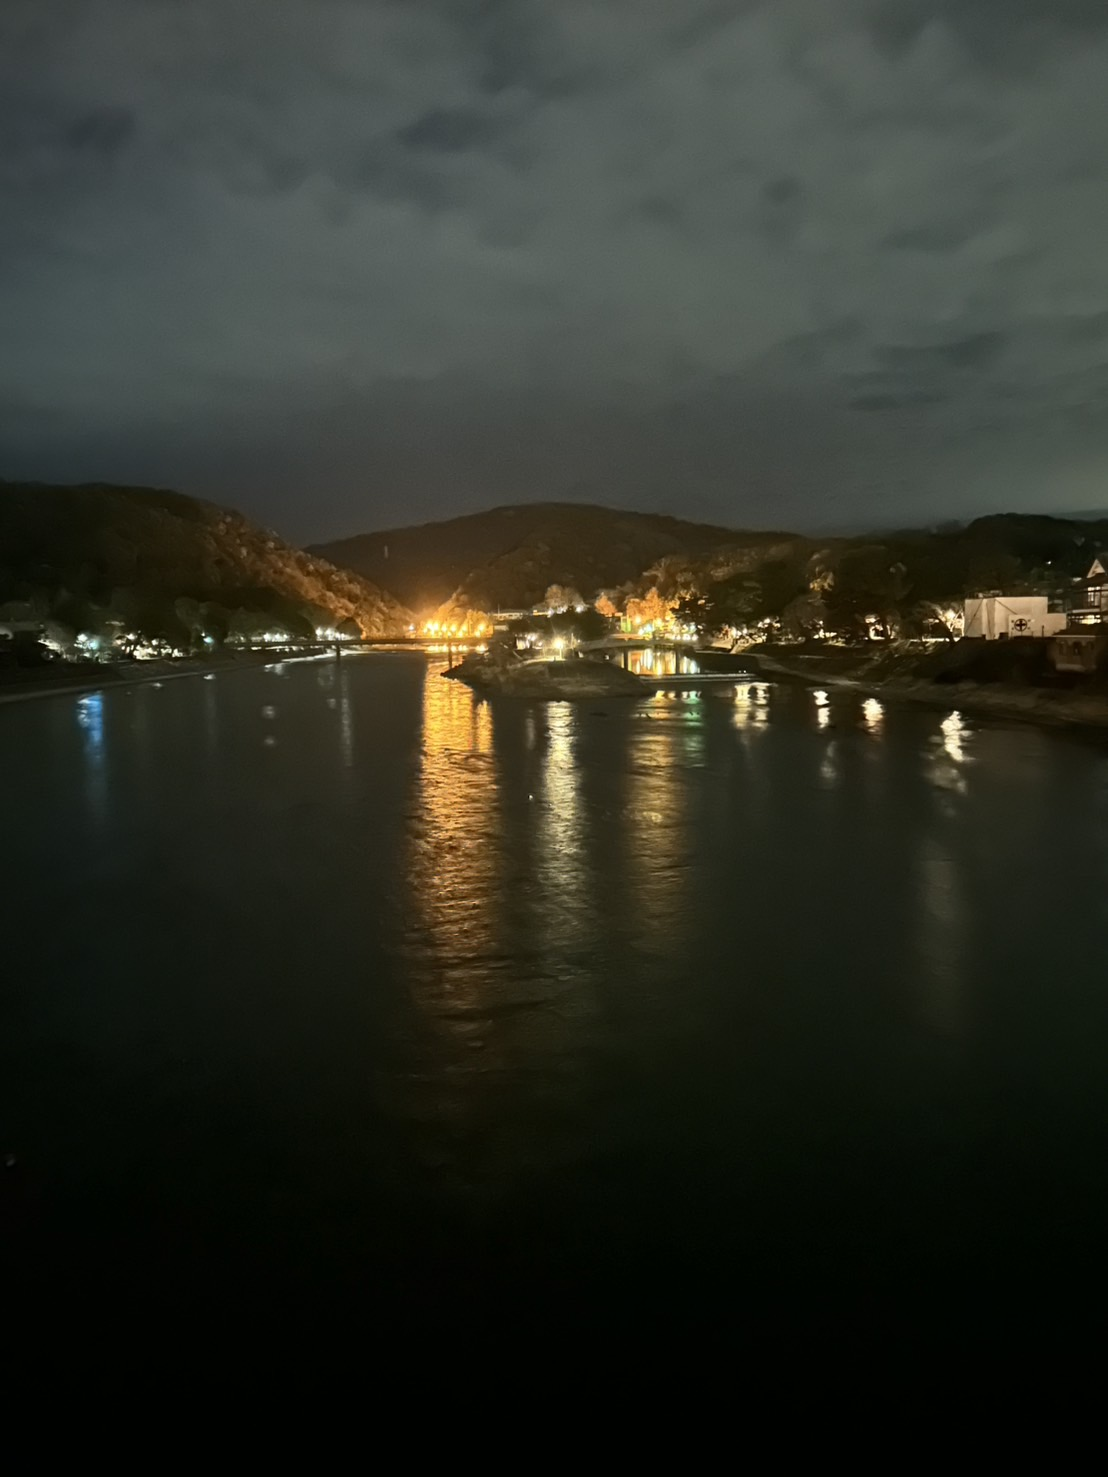
\includegraphics[width=5cm]{2025shinki/shinya_haikai/image2.png}
    \caption{@宇治川}
    \label{fig:enter-label2}
\end{figure}
深夜と川ってめちゃくちゃ良いんですよね。背景の山によるレイヤーも明かりも川への反射も良い。これで月とか写っていれば最強でした。川や湖面に映る光の揺れ加減にあらわれる各人のフェティッシュを聞くのが大好きです。

\begin{figure}[H]
    \centering
    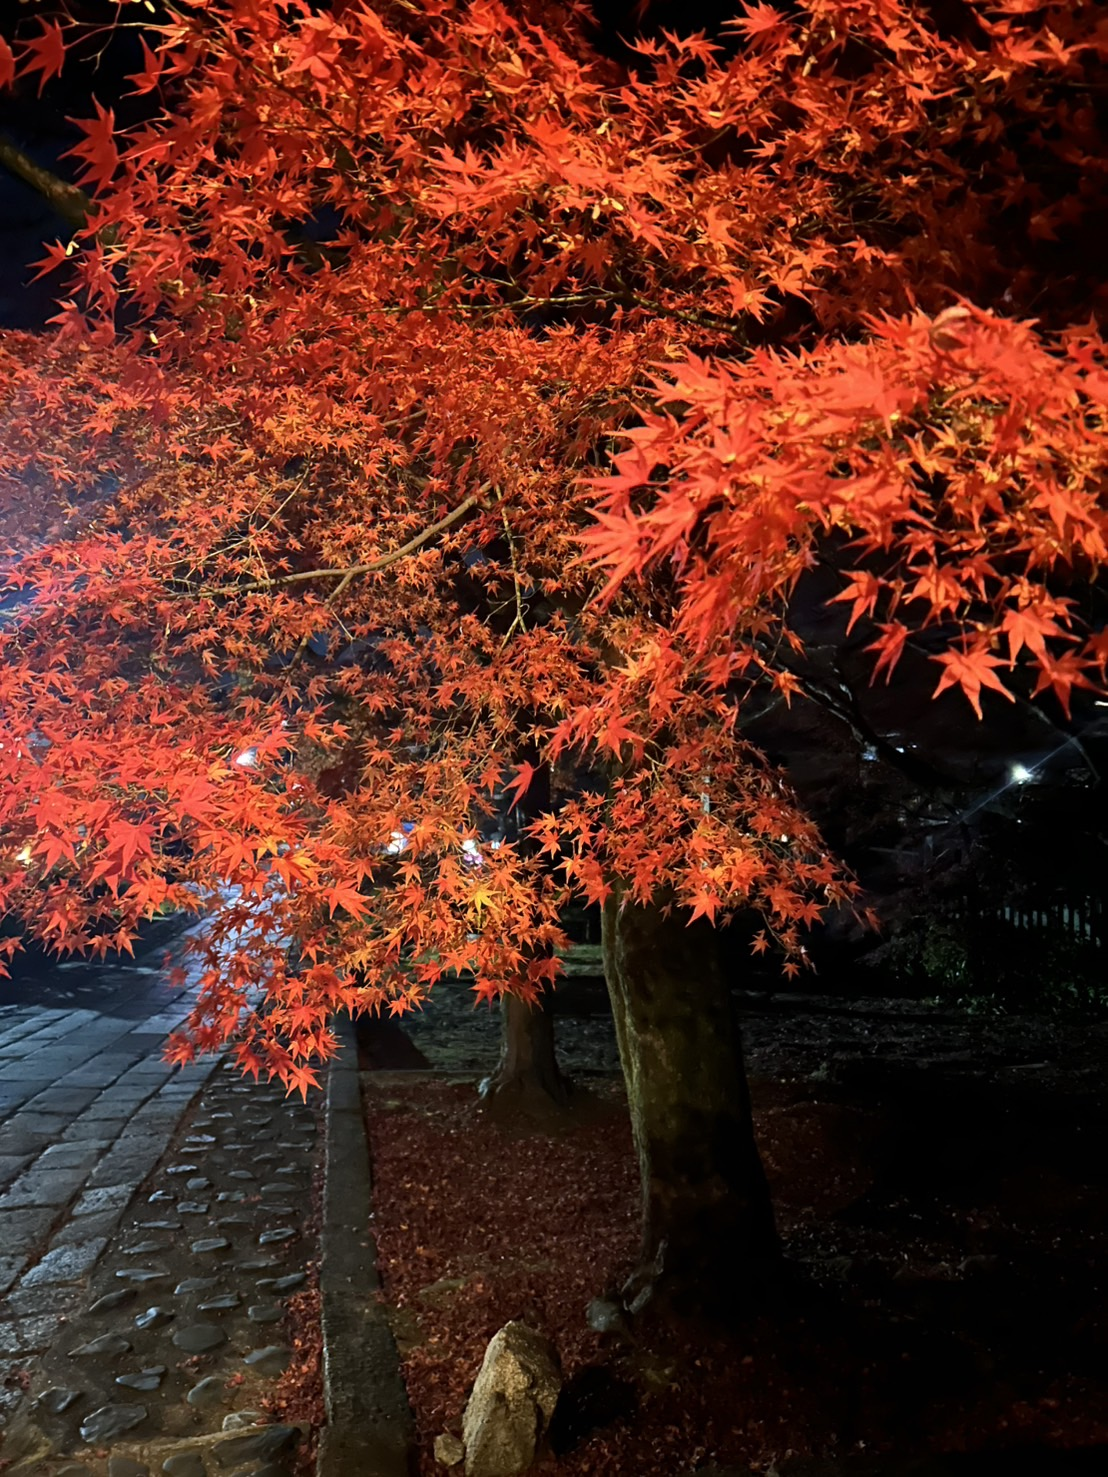
\includegraphics[width=5cm]{2025shinki/shinya_haikai/image3.png}
    \caption{もみじ}
    \label{fig:enter-label3}
\end{figure}
深夜ともみじってめちゃくちゃ良いんですよね。となりに映る道も夜であるが故の艶やかさが感じられて好みです。季節限定ですから、寒さを乗り越えてがんばって歩きましょう。新入寮生に向けて言えば夜桜もとってもおすすめなのですが、いま手元に写真がありませんでした…一緒に撮りに行きましょう!

\begin{figure}[H]
    \centering
    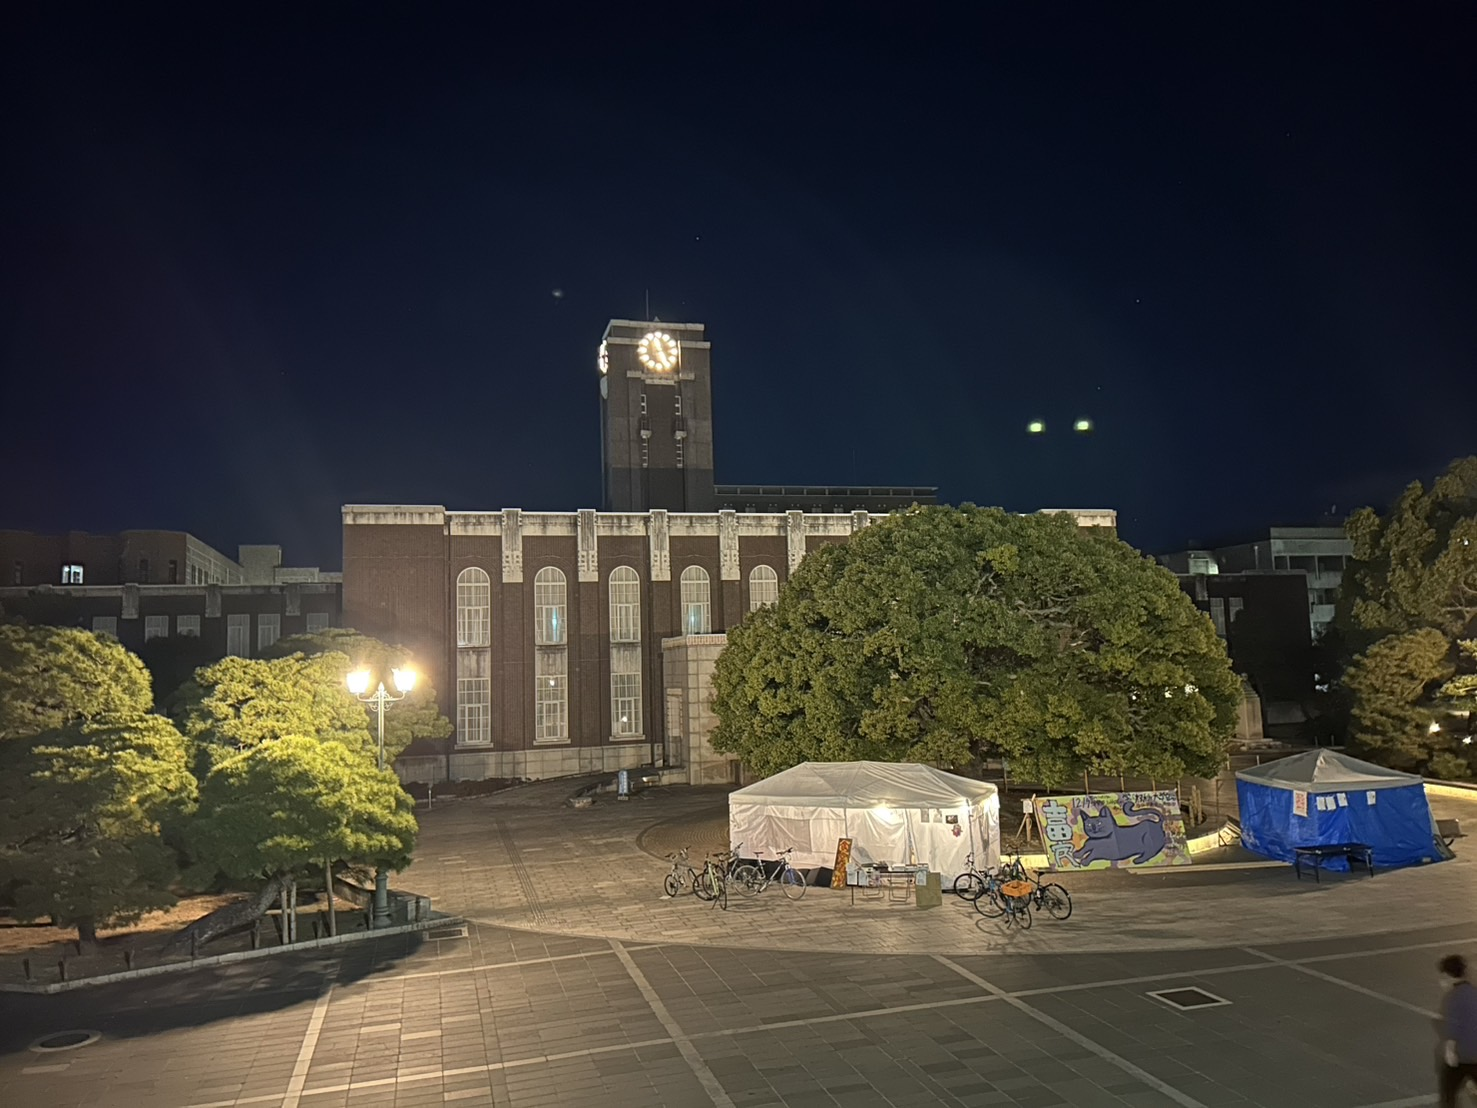
\includegraphics[width=5cm]{2025shinki/shinya_haikai/image4.png}
    \caption{@京都大学}
    \label{fig:enter-label4}
\end{figure}
京都大学に深夜に侵入すると、実はできることが多くて楽しいですよ!ここでは具体的には書きませんが、入寮後にたくさん語りたいと思います。写真中のテントは吉田寮のものですが、熊野寮でもキャンパス情宣といって、楠の前にテントを立てて夜を明かす活動を行っているので、ぜひ体験してみてください。\\ \indent

以下は部員から提供された写真になります。(紹介文もいただきました!)
\begin{figure}[H]
    \centering
    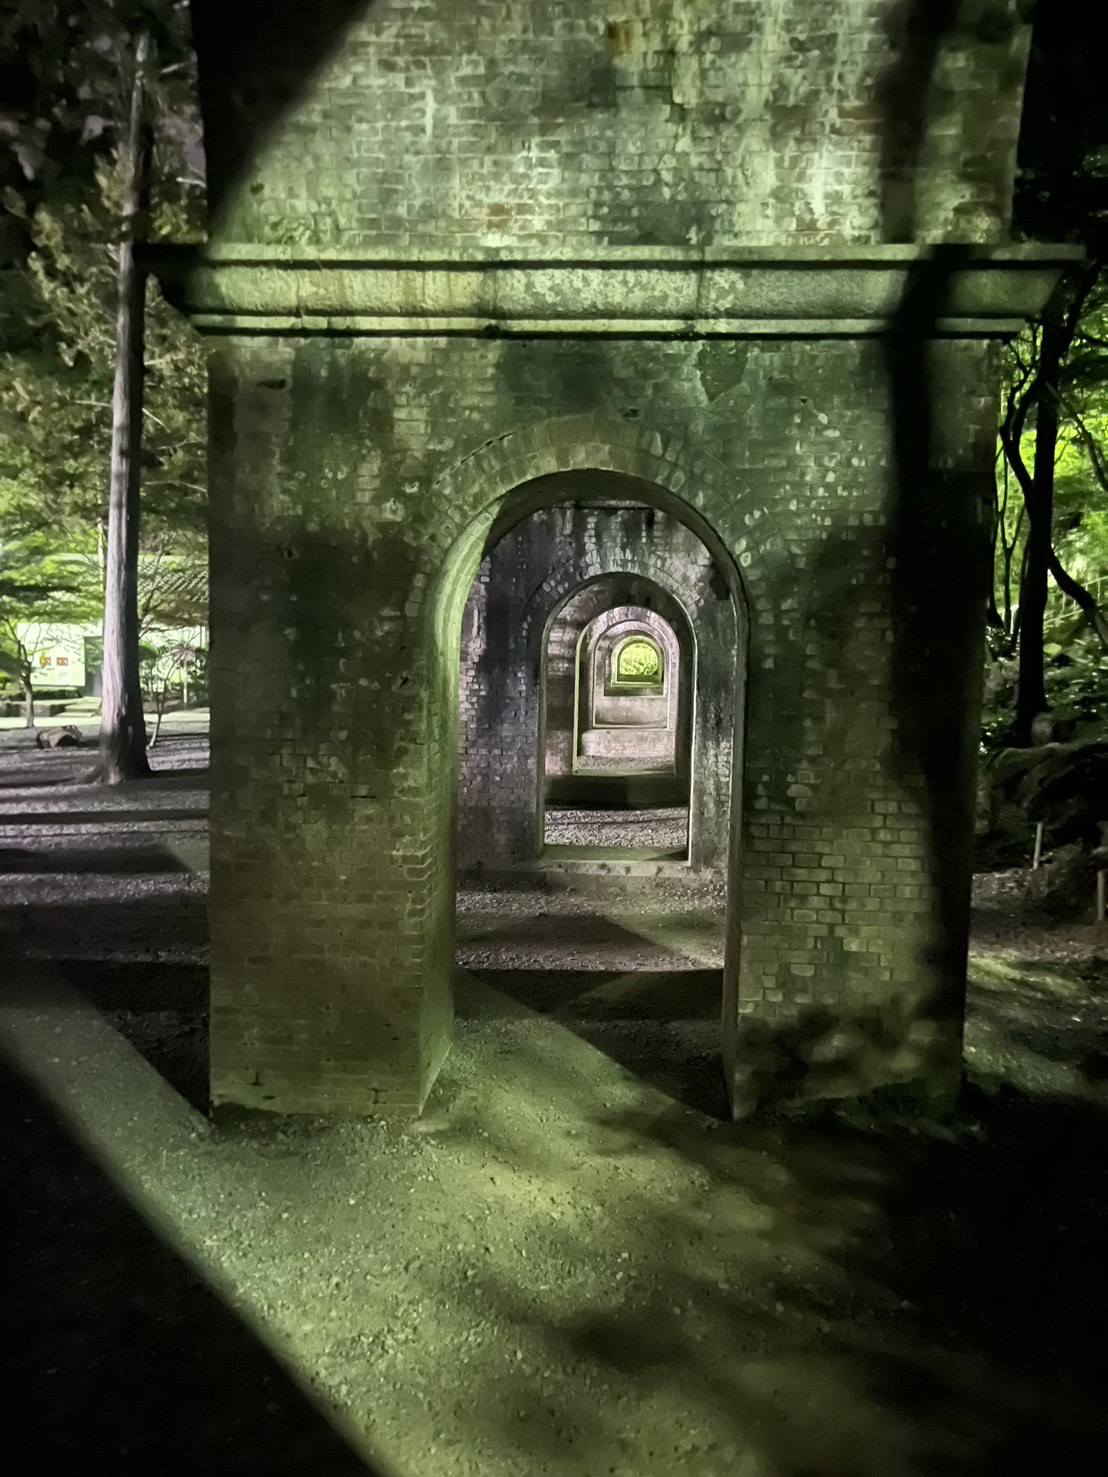
\includegraphics[width=5cm]{2025shinki/shinya_haikai/image5.png}
    \caption{南禅寺水路閣}
    \label{fig:enter-label5}
\end{figure}
人気のフォトスポットなので、知っている人もいるかもしれません。南禅寺は寮から適度に近く、深夜徘徊先として優秀です。敷地が広くて落ち着いているし、塔頭もたくさんあって、外の世界とは違うひとつの街を構成しているようでお気に入りのお寺です。昼間に行くのもいいですが、この写真のように人が一人もいない水路閣は夜しか見ることができません!周辺に植えられているもみじも綺麗で、個人的には南禅寺は紅葉より青もみじが好きです。


\begin{figure}[H]
    \centering
    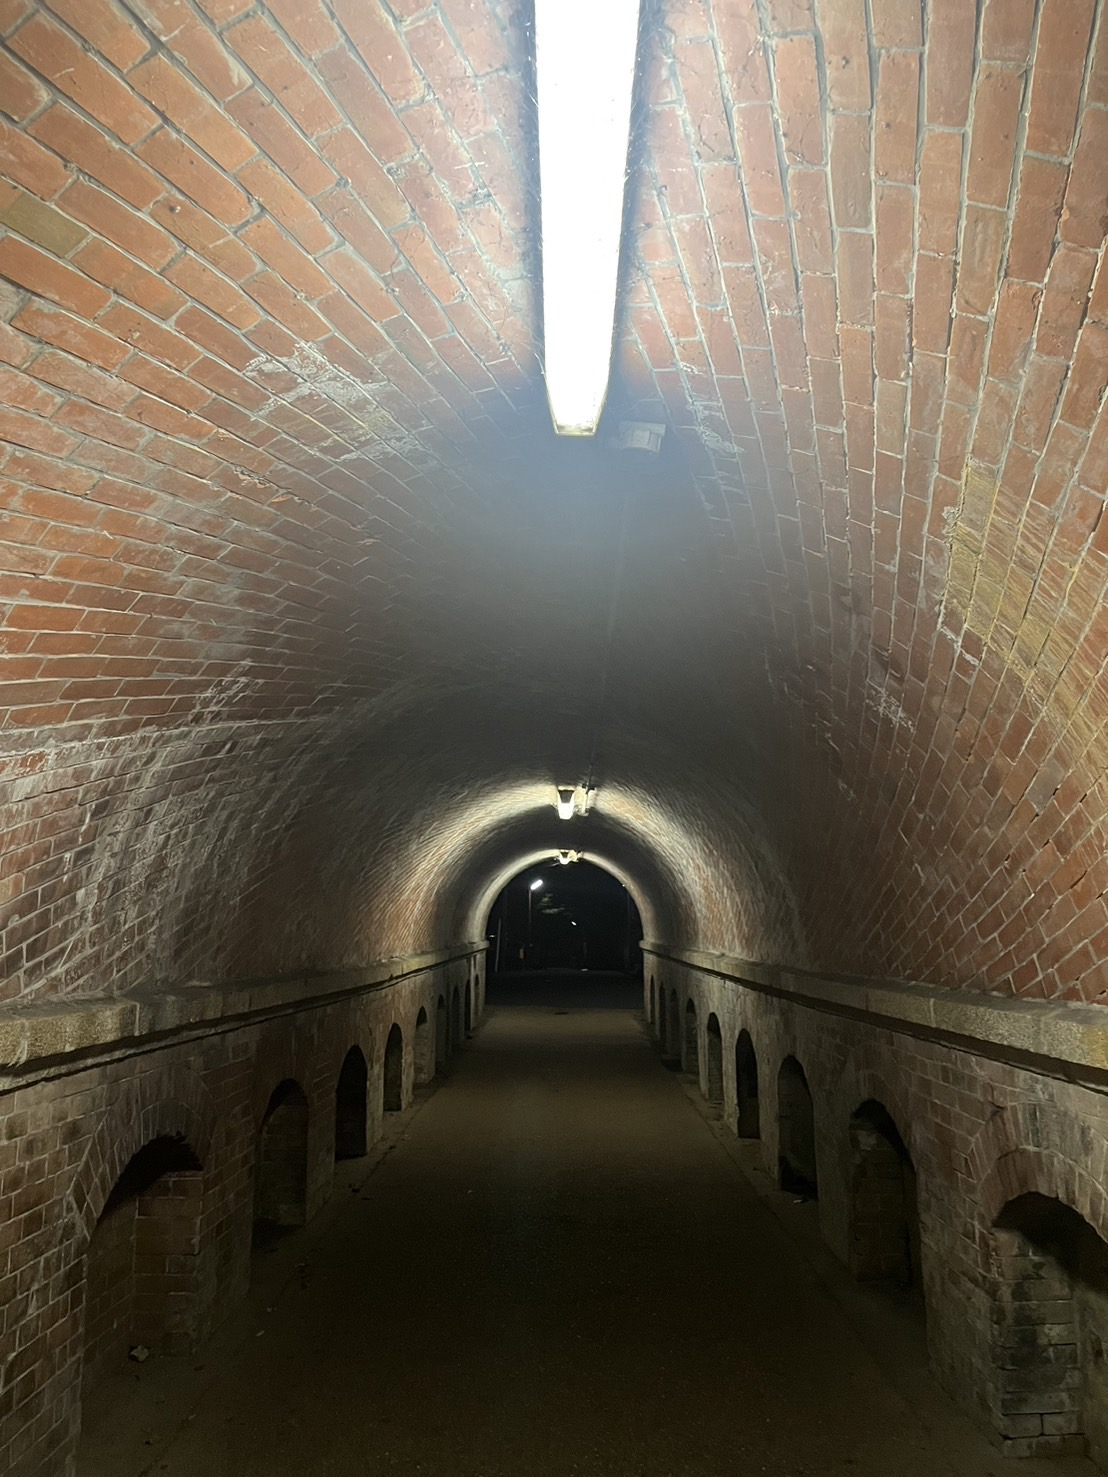
\includegraphics[width=5cm]{2025shinki/shinya_haikai/image6.png}
    \caption{琵琶湖疏水ねじりまんぽ}
    \label{fig:enter-label6}
\end{figure}
ここも南禅寺界隈です。「ねじりまんぽ」というのは「ねじりのあるトンネル」を意味しています。螺旋状に煉瓦を積み上げることで強度を確保しているそうです。トンネルってある世界とある世界を分ける役割を果たしていると思うんですが、このトンネルもそれに漏れず、落ち着いた、どこか異世界感のある南禅寺と多くの車が行き交う三条通とをくっきりと分けています。また、煉瓦が螺旋状に配置されていることで、より違う世界に行く感覚が強くなっている気がします。


\subsection{おわりに}
やっと書き終わりました(午前3時)。乱文で申し訳ありません。深夜徘徊部にもかかわらず普通に眠いです、いまから寝ます。著しく締め切りを過ぎての寄稿に謝罪するとともに、編集してくれる皆さんに感謝を申し上げて結びとしたいと思います。読んでくれた皆さん、また話しましょうね~~~~
